\chapter{Etat d'avancement}
\section{Fonctionnalités développées}
À la fin ce projet, nous sommes arrivés à produire une application fonctionnelle qui permet de:\bigskip

\begin{itemize}
 	\item créer, supprimer et modifier des parcours
 	\item créer, supprimer des trajets
 	\item enregistrer les coordonnées GPS du trajet 
 	\item afficher le trajet sur une carte avec son trajet de référence
 	\item définir un trajet comme référence du parcours
	\item consulter l'historique des trajets 
	\item consulter les différentes statistiques relatives aux parcours 
	\begin{itemize}
		\item la vitesse moyenne
		\item l'allure moyenne
		\item le temps moyen 
		\item les meilleurs temps et vitesse 
	\end{itemize}
 	\item consulter les différentes statistiques relatives aux trajets 
	\begin{itemize}
		\item la vitesse
		\item la distance parcourue
		\item l'allure
		\item le temps du trajet 
	\end{itemize}
\end{itemize}\bigskip

\newpage

\section{Design de l'application}
Voici à quoi ressemble l'application terminée:\bigskip 

\begin{multicols}{2}
\begin{img}
  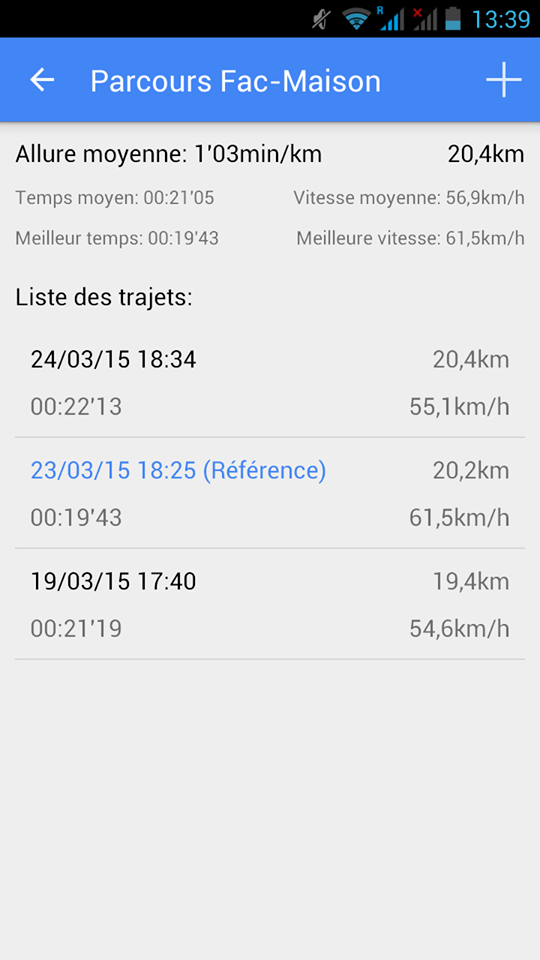
\includegraphics[scale=0.35]{img/parcours.jpg}
  \caption{Détail d'un parcours}
  \label{détail Parcours}
\end{img}
\begin{img}
  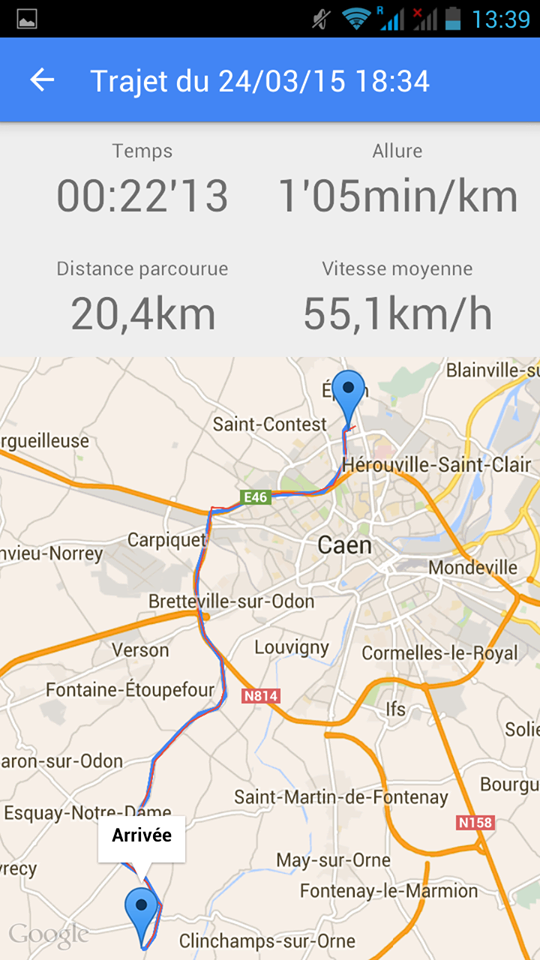
\includegraphics[scale=0.35]{img/trajet.jpg}
  \caption{Détail d'un trajet}
  \label{détail trajet}
\end{img}
\end{multicols}

Dans l'écran de détail d'un parcours (figure \ref{détail Parcours}) le parcours nommé "Fac-Maison" contient trois trajets triés par ordre anti-chronologique. Le second parcours est défini comme trajet de référence.\bigskip

Sur la carte du détail du trajet (figure \ref{détail trajet}), le trajet consulté est tracé en bleu et le trajet de référence en rouge. Cela permet à l'utilisateur de déceler les éventuels écarts de parcours tout au long du trajet.\bigskip

D'autres captures d'écran sont disponibles dans l'annexe \ref{Annexe4}.